\chapter{Real Life Case Study of CCRK-Related Cancers}

% \cite{1384} Some freely accessible drug databases include DrugBank,43 e-Drug 3D,44 KEGG DRUG45 and the superdrug database.46
% \cite{1384} Miteva and co-workers have used normal mode analysis to choose relevant conformations appropriate for subsequent ligand docking using cyclic dependent receptor kinase 2 (CDK2) as a model structure.63
% \cite{1384} 76 In their study, the authors examined the utility of IFPs as post-docking filters for the screening of CDK2 inhibitors using four different docking algorithms (FlexX, Gold, glide, and Surflex) and the Tanimoto metric (Tc-IFP) to evaluate the similarity of the predicted X-ray IFP to the re-docked pose.

\section{Background}

CCRK (Cell Cycle-Related Kinase), also known as p42, CDK-related kinase PNQALRE, or CDK20, is a newly identified 42kDa protein containing all 11 conserved subdomains characteristic of serine/threonine protein kinase.

Prof. Marie Chia-Mi Lin and her team from Department of Surgery at Prince of Wales Hospital investigated the involvement of CCRK in glioblastoma multiforme carcinogenesis. They analyzed the expression levels of CCRK in 26 glioma patient samples and normal brain, and observed that 1) knock down of CCRK by siRNA (small-interfering RNA) inhibited glioblastoma cell proliferation, 2) suppression of CCRK by shRNA (short hairpin RNA) inhibited glioblastoma tumor growth in nude mice, and 3) CCRK overexpression conferred tumorigenicity to a non-tumorigenic U-138 cell line, and concluded CCRK to be a candidate oncogene in glioblastoma multiforme tumorigenesis \citep{1144}.

Moreover, they examined CCRK expression in a series of ovarian carcinoma tissues by immunohistochemistry, and detected overexpression of CCRK in 53\% of the ovarian carcinomas, and found it positively correlated with patients' clinicopathological characteristics \citep{1145}. They also investigated the role of CCRK in human colorectal cancer carcinogenesis, and found that CCRK protein levels were elevated by more than 1.5-fold in 70\% of colorectal cancer patient samples examined and CCRK was detectable in all seven colorectal cancer cell lines tested \citep{1143}. Suppression of CCRK by siCCRK led to G1 phase cell cycle arrest and reduced cell growth. CCRK is required for the phosphorylation of CDK2 (Cyclin-Dependent Kinase 2) on Thr160 and Rb on Ser795 and the expression of cyclin E \citep{1143}. 

Furthermore, together with Prof. Joseph Jao-Yiu Sung's team, they used genome-wide location and functional analyses to identify CCRK as a direct androgen receptor-regulated gene that drives $\beta$-catenin/T cell factor-dependent hepatocarcinogenesis \citep{1146}. Conversely, knock down of CCRK decreased hepatocellular carcinoma cell growth. CCRK overexpression correlated with the tumor staging and poor overall survival of patients \citep{1146}.

They therefore attempted to seek for CCRK inhibitors for the treatment of cancers and drug resistances. Due to the absence of CCRK structure in the PDB database \citep{540,537}, they utilized Chem3D from the then CambridgeSoft company, now acquired by PerkinElmer, Inc., to build a homologous model of CCRK from CDK2 based on the fact that they share 35\% sequence identity (Figure \ref{Case:CDKAlignment}), and performed protein-ligand docking of TCMs (Traditional Chinese Medicines) with AutoDock 3.0.5 and Cerius2 LigandFit, and identified 22-O-Angeloyl theasapogenol B (PubChem CID 5318850) as a potential potent inhibitor that could fit into the deep and narrow active site of their homologous model of CCRK. It was, nevertheless, very difficult to purify the compound from puerh tea.

\begin{figure}
\centering
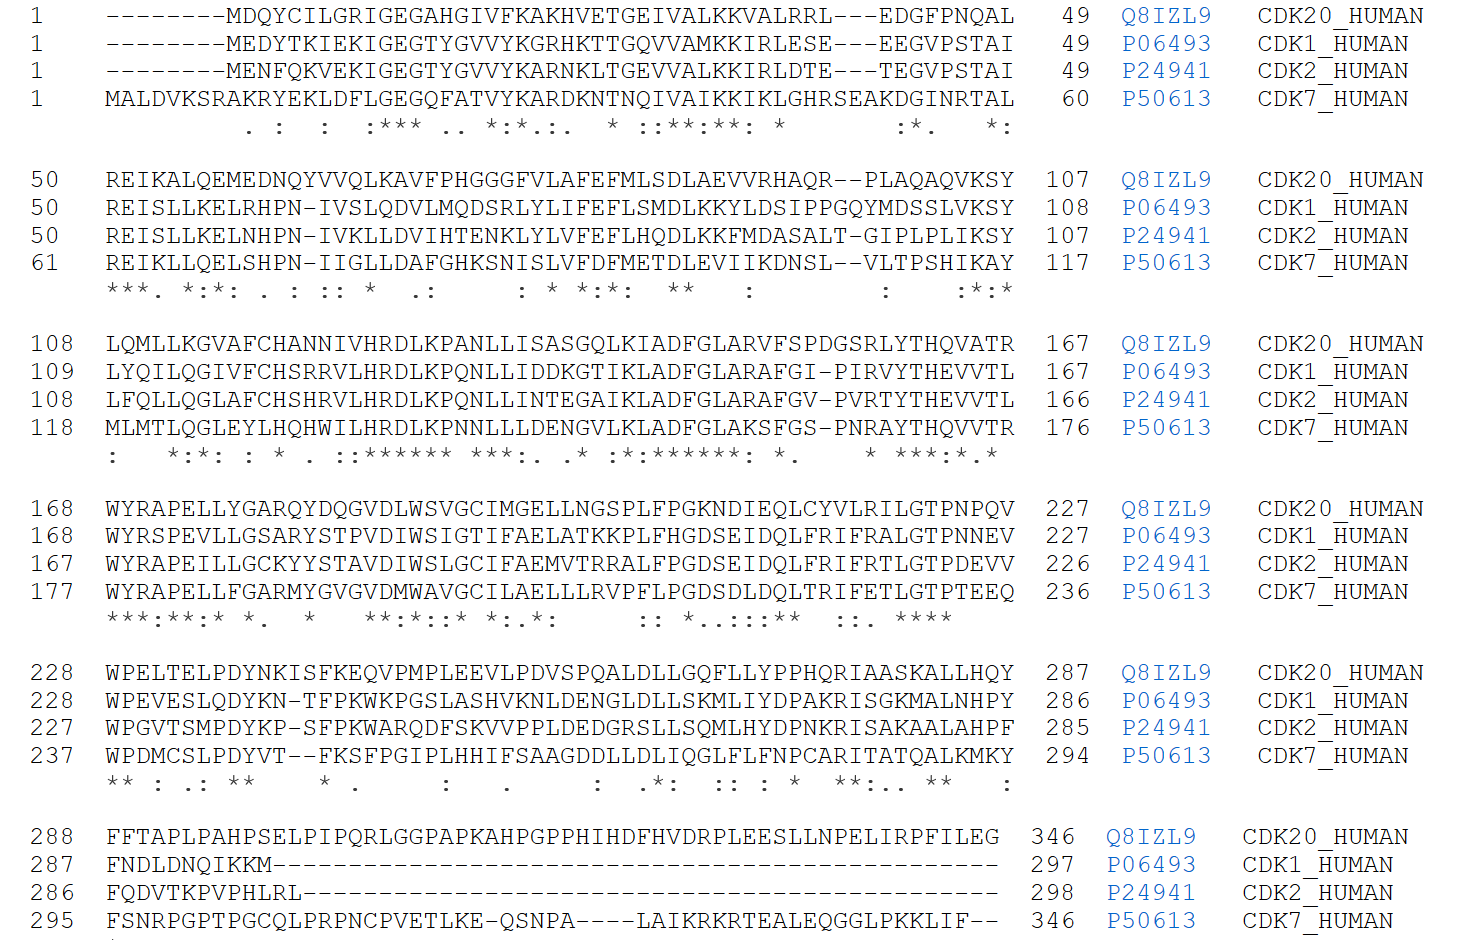
\includegraphics[width=\linewidth]{../ccrk/CDKAlignment.png}
\caption{Protein sequence alignment of CDK20, CDK1, CDK2 and CDK7.}
\label{Case:CDKAlignment}
\end{figure}

\section{Our Contributions}

We are collaborating with Prof. Lin's team on identifying inhibitors of CCRK. We used as receptor the CCRK homologous model (Figure \ref{Case:CCRKHomologousModel}) built by Dr. William Cheung based on the CDK2 template with PDB ID 1HCL \citep{1142} using SWISS-MODEL, a fully automated protein structure homology-modeling server accessible via the ExPASy web server. We concentrated on repurposing approved drugs \citep{944,1023} because developing a drug \textit{de novo} is a laborious and costly endeavor. Using idock 1.5 with a fine grid map granularity of 0.08\AA\ and 512 Monte Carlo tasks, we screened 1,715 FDA-approved drugs via DrugBank and 3,176 FDA-approved drugs via DSSTOX. Figures \ref{Case:1HCL-ZINC03830332} and \ref{Case:1HCL-ZINC03831625} depict the interactions between the CCRK homologous model and two high-rank ligands.

\begin{figure}
\centering
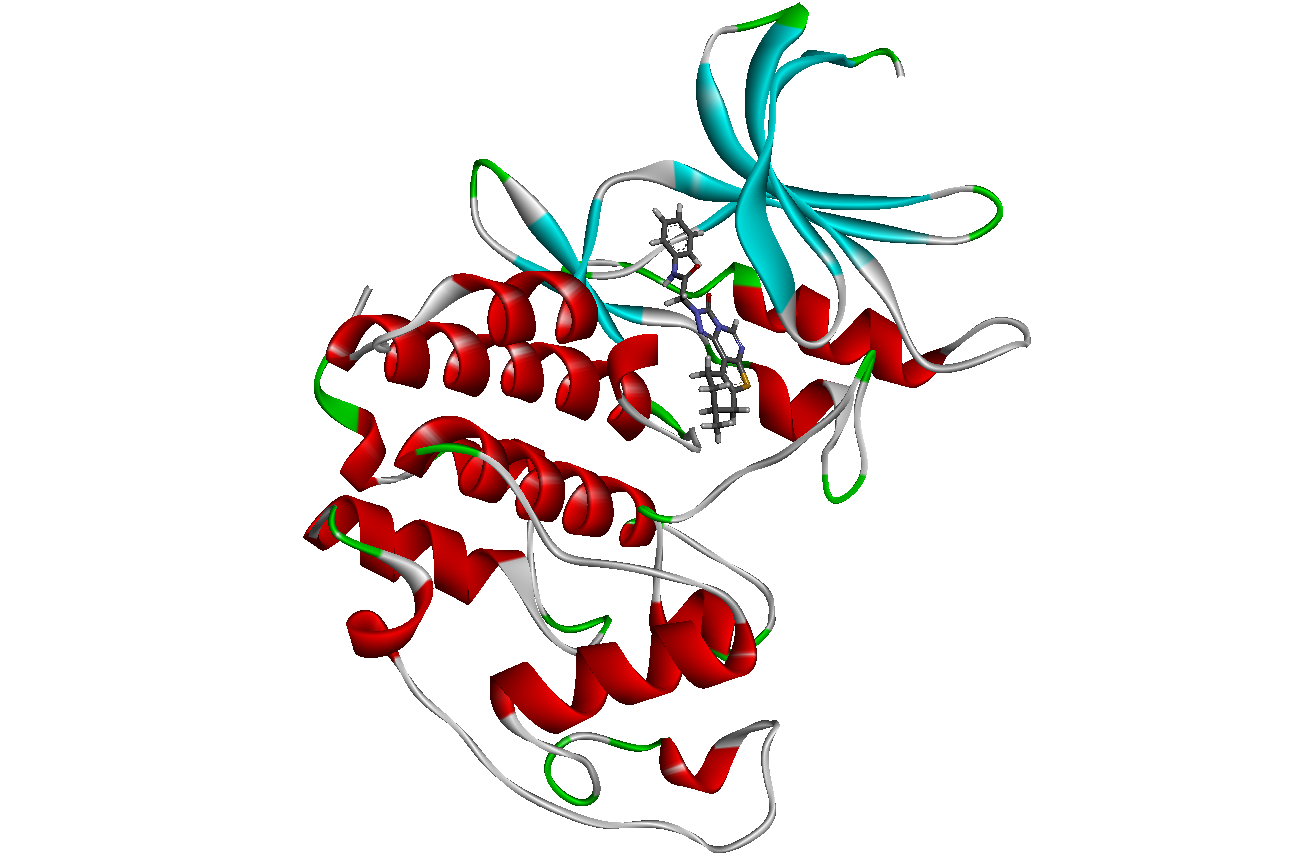
\includegraphics[width=\linewidth]{../ccrk/CCRKHomologousModel.png}
\caption{CCRK homologous model, built by Dr. William Cheung based on the CDK2 template with PDB ID 1HCL \citep{1142} using SWISS-MODEL. The ligand denotes the Ser/Thr protein kinase active site.}
\label{Case:CCRKHomologousModel}
\end{figure}

\begin{figure}
\centering
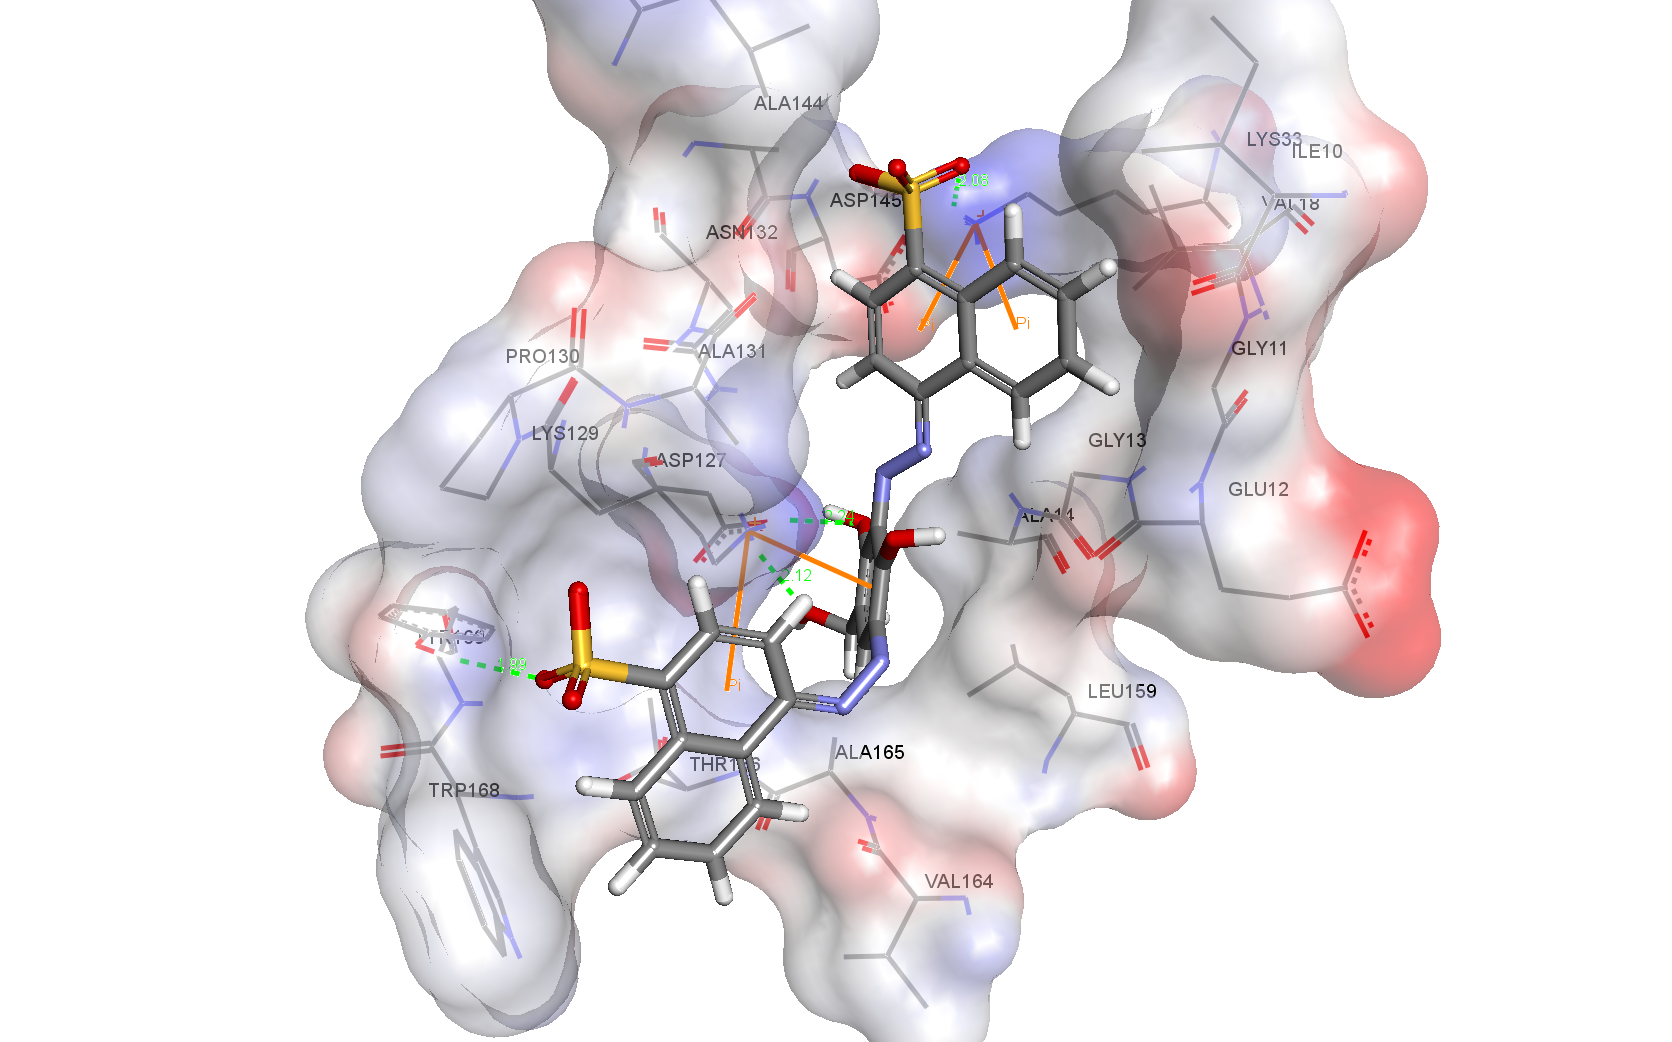
\includegraphics[width=\linewidth]{../ccrk/1HCL-ZINC03830332.png}
\caption{CCRK homologous model in complex of ZINC03830332, which forms 4 hydrogen bonds with LYS33, LYS129 and TYR169, and Pi-Cation interactions with LYS33 and LYS129. Free energy predicted by idock is -10.306 kcal/mol.}
\label{Case:1HCL-ZINC03830332}
\end{figure}

\begin{figure}
\centering
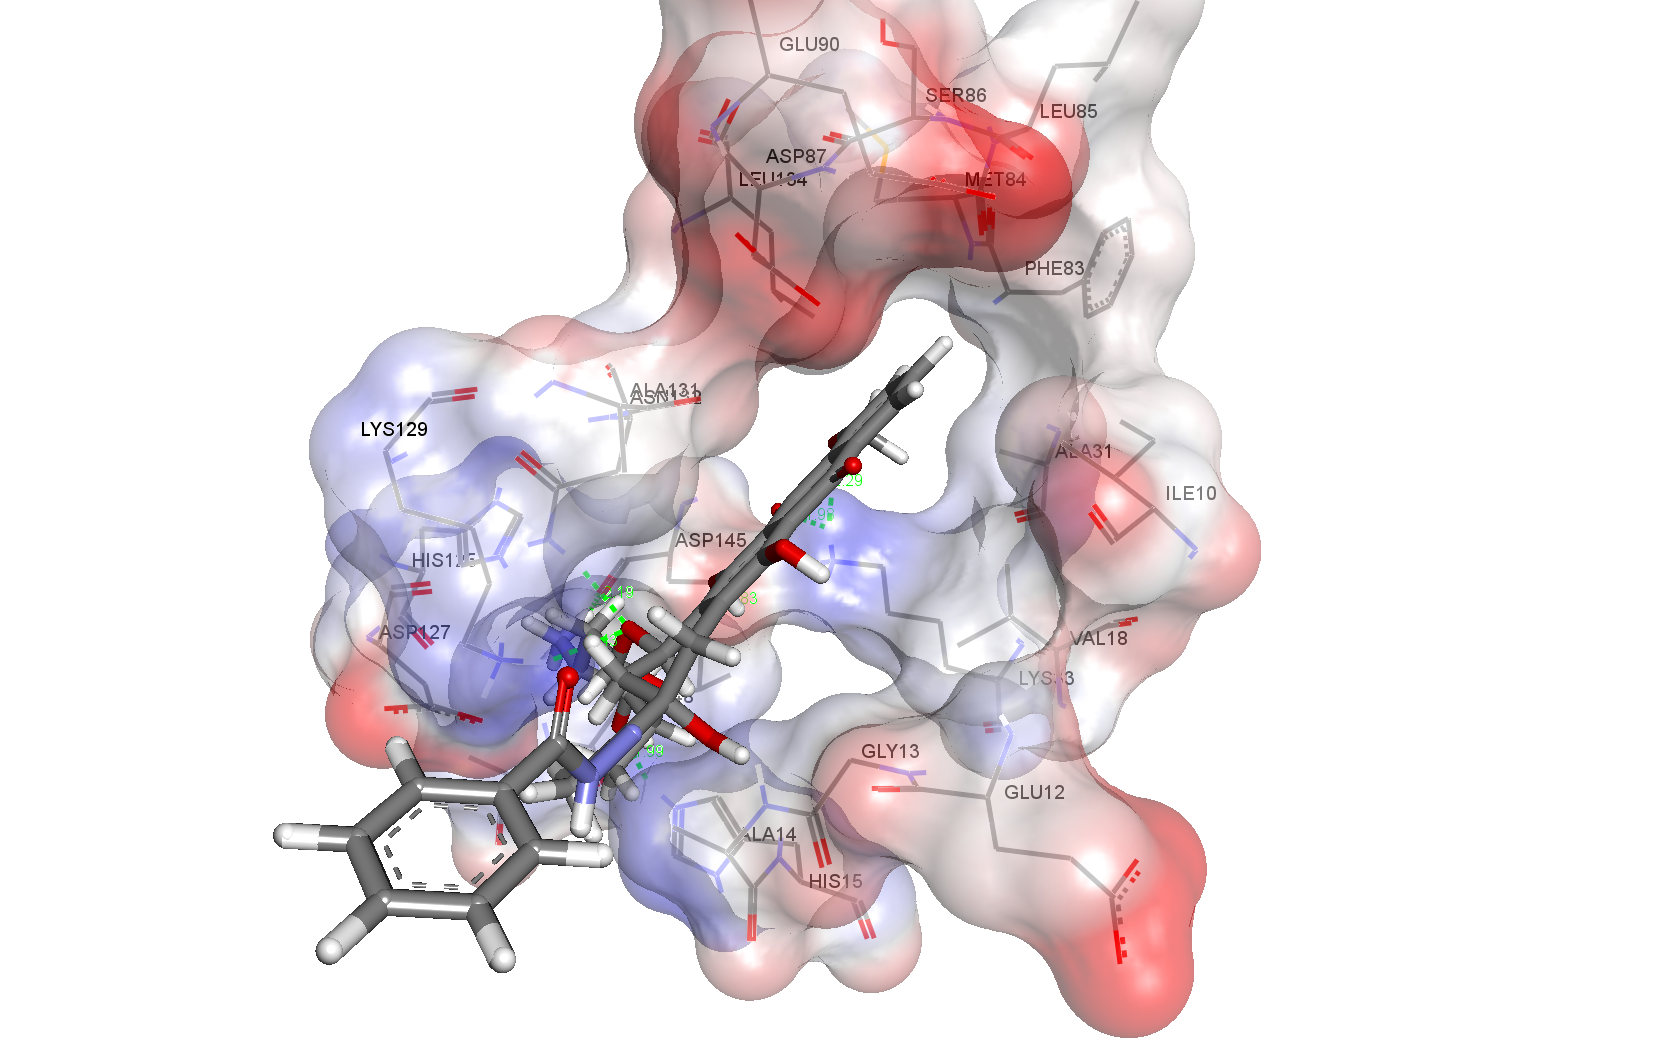
\includegraphics[width=\linewidth]{../ccrk/1HCL-ZINC03831625.png}
\caption{CCRK homologous model in complex of ZINC03831625, which forms 7 hydrogen bonds with HIS15, LYS33, LYS129, ASN132 and ASP145. Free energy predicted by idock is -9.438 kcal/mol.}
\label{Case:1HCL-ZINC03831625}
\end{figure}

\chapterend
